\section{R-Baum 2}
%% Vorlagen für die Zeichnungen
% circle radius
\newdimen\R
\R=0.5cm

\newcommand{\nodeAA} {
	\draw (4.5, 4.5) circle (\R) node {A};
}
\newcommand{\nodeBB} {
	\draw[xshift=1.0cm,yshift=3.3cm] (0:\R) \foreach \x in {72,144,...,359} {
		-- (\x:\R)
	} -- cycle (0:\R) node {B \hspace{0.8cm} } ;
}
\newcommand{\nodeCC} {
	\draw[xshift=0.8cm,yshift=1.7cm] (0:\R) \foreach \x in {120,240} {
		-- (\x:\R)
	} -- cycle (0:\R) node {C \hspace{0.9cm} } ;
}
\newcommand{\nodeDD} {
	\draw (0.7  , 4.5) circle (\R) node {D};
}
\newcommand{\nodeEE} {
	\draw (5.0, 1.0) circle (\R) node {E};
}
\newcommand{\nodeFF} {
	\draw[xshift=5.2cm,yshift=2.1cm] (0:\R) \foreach \x in {120,240} {
		-- (\x:\R)
	} -- cycle (0:\R) node {F \hspace{0.9cm} } ;
}
\newcommand{\nodeGG} {
	\draw (5.1, 3.3) circle (\R) node {G};
}
\newcommand{\nodeHH} {
	\draw (1.8, 5.3) circle (\R) node {H};
}
\newcommand{\nodeII} {
	\draw (1.9, 0.7) circle (\R) node {I};
}
\newcommand{\nodeJJ} {
	%\draw (2.4, 3.8) circle (\R) node {J};
	\draw[xshift=2.4cm,yshift=3.8cm] (0:\R) \foreach \x in {120,240} {
		-- (\x:\R)
	} -- cycle (0:\R) node {J \hspace{0.9cm} } ;
}


\newcommand{\RAA} {
	\draw (4  , 4  ) rectangle (5  , 5  ) node[pos=0.9,anchor=south east] {R1};
}
\newcommand{\RBB} {
	\draw (0.56, 2.8) rectangle (1.5, 3.8) node[pos=0.1,anchor=south east] {R2};
}
\newcommand{\RCC} {
	\draw (0.52, 2.2) rectangle (1.3, 1.2) node[pos=0.9,anchor=north east] {R3};
}
\newcommand{\RDD} {
	\draw (0.2, 4.0) rectangle (1.2, 5.0) node[pos=0.1,anchor=south east] {R4};
}
\newcommand{\REE} {
	\draw (4.5, 0.5) rectangle (5.5, 1.5) node[pos=0.1,anchor=north east] {R5};
}
\newcommand{\RFF} {
	\draw (4.92, 2.6) rectangle (5.7, 1.6) node[pos=0.2,anchor=north east] {R8};
}
\newcommand{\RGG} {
	\draw (4.6, 2.8) rectangle (5.6, 3.8) node[pos=0.2,anchor=north east] {R9};
}
\newcommand{\RHH} {
	\draw (1.3, 4.8) rectangle (2.3, 5.8) node[pos=0.9,anchor=north west] {R10};
}
\newcommand{\RII} {
	\draw (1.4, 0.2) rectangle (2.4, 1.2) node[pos=0.9,anchor=north west] {R11};
}
\newcommand{\RJJ} {
	\draw (2.12, 4.3) rectangle (2.9, 3.3) node[pos=0.9,anchor=north west] {R12};
}


Gegeben sei ein anfangs leerer R-Baum mit $M=4$ sowie die geometrischen Objekte A bis J im zweidimensionalen Raum.
Des Weiteren s wieder $m = \lfloor\frac{M}{2}\rfloor$:

\begin{center}
	\begin{tikzpicture}
		% border
		\draw (0,0) rectangle (6,6);

		\nodeAA
		\nodeBB
		\nodeCC
		\nodeDD
		\nodeEE
		\nodeFF
		\nodeGG
		\nodeHH
		\nodeII
		\nodeJJ

		%\RAA
		%\RBB
		%\RCC
		%\RDD
		%\REE
		%\RFF
		%\RGG
		%\RHH
		%\RII
		%\RJJ

	\end{tikzpicture}
\end{center}

\begin{enumerate}[a)]
	\item Fügen Sie die Einträge A bis E ein.

	\begin{note}
		Zunächst wird nur der Wurzelknoten gefüllt:
		\begin{center}
			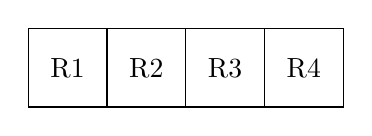
\begin{tikzpicture}
				\draw (0,0) rectangle (1,1) node[pos=.5] {R1};
				\draw (1,0) rectangle (2,1) node[pos=.5] {R2};
				\draw (2,0) rectangle (3,1) node[pos=.5] {R3};
				\draw (3,0) rectangle (4,1) node[pos=.5] {R4};
			\end{tikzpicture}
		\end{center}

		Die minimalen Rechtecke:
		\begin{center}
			\begin{tikzpicture}
				% border
				\draw (0,0) rectangle (6,6);

				\nodeAA
				\nodeBB
				\nodeCC
				\nodeDD

				\RAA
				\RBB
				\RCC
				\RDD
			\end{tikzpicture}
		\end{center}

		Durch E erfolgt der erste Splitt:


		Die minimalen Rechtecke:
		\begin{center}
			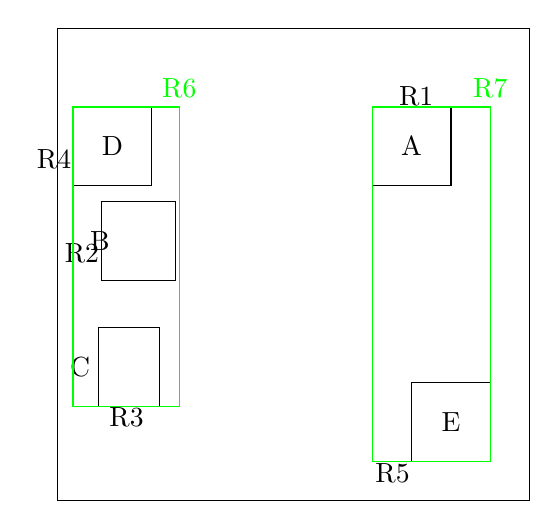
\begin{tikzpicture}
				% border
				\draw (0,0) rectangle (6,6);

				\nodeAA
				\nodeBB
				\nodeCC
				\nodeDD
				\nodeEE

				\RAA
				\RBB
				\RCC
				\RDD
				\REE

				% root node
				\draw[color=green] (0.2  , 1.2) rectangle (1.55, 5  ) node[anchor=south] {R6};
				\draw[color=green] (4.0, 0.5) rectangle (5.5, 5.0) node[anchor=south] {R7};
			\end{tikzpicture}
		\end{center}

		\begin{center}
			\begin{tikzpicture}
				\draw (-1.5,0) rectangle (-0.5,1) node[name=R6,pos=.5] {R6};
				\draw (-0.5,0) rectangle (0.5,1) node[name=R7,pos=.5] {R7};
				\draw (0.5,0) rectangle (1.5,1) node[name=D1,pos=.5] {};
				\draw (1.5,0) rectangle (2.5,1) node[name=D2,pos=.5] {};

				\draw (-5,-2) rectangle (-4,-1) node[name=R1,pos=.5] {R2};
				\draw (-4,-2) rectangle (-3,-1) node[name=R3,pos=.5] {R3};
				\draw (-3,-2) rectangle (-2,-1) node[name=R5,pos=.5] {R4};
				\draw (-2,-2) rectangle (-1,-1) node[name=D3,pos=.5] {};

				\draw (1,-2) rectangle (2,-1) node[name=R2,pos=.5] {R1};
				\draw (2,-2) rectangle (3,-1) node[name=R4,pos=.5] {R5};
				\draw (3,-2) rectangle (4,-1) node[name=D4,pos=.5] {};
				\draw (4,-2) rectangle (5,-1) node[name=D5,pos=.5] {};

				\node[fit=(R1)(R3)(R5)(D3)](leftLeaf){};
				\node[fit=(R2)(R4)(D4)(D5)](rightLeaf){};

				\draw [thick, ->, >=stealth']
				([yshift=-2.5mm]R6.south) -- ([yshift=1mm]leftLeaf.north);
				\draw [thick, ->, >=stealth']
				([yshift=-2.5mm]R7.south) -- ([yshift=1mm]rightLeaf.north);
			\end{tikzpicture}
		\end{center}

	\end{note}

	\item
	Löschen sie anschließend den Eintrag B.

	\begin{note}
		Der Knoten B, bzw. das minimale umgebende Rechteck R2, werden aus dem linken Blattknoten entfernt. Bei diesem Löschvorgang entsteht kein Unterlauf.
		\begin{center}
			\begin{tikzpicture}
				\draw (-1.5,0) rectangle (-0.5,1) node[name=R6,pos=.5] {R6};
				\draw (-0.5,0) rectangle (0.5,1) node[name=R7,pos=.5] {R7};
				\draw (0.5,0) rectangle (1.5,1) node[name=D1,pos=.5] {};
				\draw (1.5,0) rectangle (2.5,1) node[name=D2,pos=.5] {};

				\draw (-5,-2) rectangle (-4,-1) node[name=R1,pos=.5] {R3};
				\draw (-4,-2) rectangle (-3,-1) node[name=R3,pos=.5] {R4};
				\draw (-3,-2) rectangle (-2,-1) node[name=R5,pos=.5] {};
				\draw (-2,-2) rectangle (-1,-1) node[name=D3,pos=.5] {};

				\draw (1,-2) rectangle (2,-1) node[name=R2,pos=.5] {R1};
				\draw (2,-2) rectangle (3,-1) node[name=R4,pos=.5] {R5};
				\draw (3,-2) rectangle (4,-1) node[name=D4,pos=.5] {};
				\draw (4,-2) rectangle (5,-1) node[name=D5,pos=.5] {};

				\node[fit=(R1)(R3)(R5)(D3)](leftLeaf){};
				\node[fit=(R2)(R4)(D4)(D5)](rightLeaf){};

				\draw [thick, ->, >=stealth']
				([yshift=-2.5mm]R6.south) -- ([yshift=1mm]leftLeaf.north);
				\draw [thick, ->, >=stealth']
				([yshift=-2.5mm]R7.south) -- ([yshift=1mm]rightLeaf.north);
			\end{tikzpicture}
		\end{center}

		Die minimalen Rechtecke:
		\begin{center}
			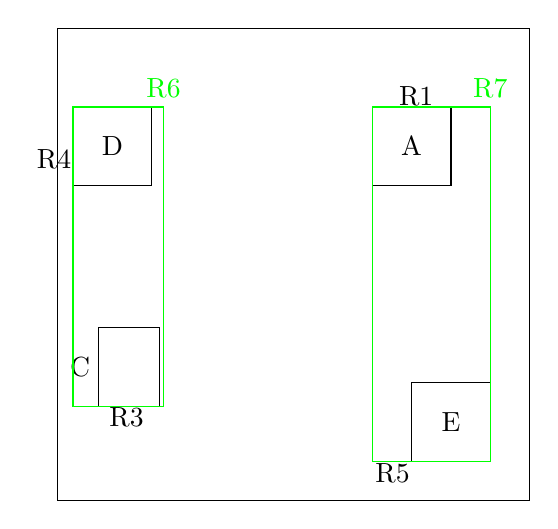
\begin{tikzpicture}
				% border
				\draw (0,0) rectangle (6,6);

				\nodeAA
				\nodeCC
				\nodeDD
				\nodeEE

				\RAA
				\RCC
				\RDD
				\REE

				% root node
				\draw[color=green] (0.2  , 1.2) rectangle (1.35, 5) node[anchor=south] {R6};
				\draw[color=green] (4.0, 0.5) rectangle (5.5, 5.0) node[anchor=south] {R7};
			\end{tikzpicture}
		\end{center}
	\end{note}

	\item
	Fügen sie anschließend die Einträge F bis J ein.

	\begin{note}
		Einfügen von Eintrag F:
		\begin{center}
			\begin{tikzpicture}
				\draw (-1.5,0) rectangle (-0.5,1) node[name=R6,pos=.5] {R6};
				\draw (-0.5,0) rectangle (0.5,1) node[name=R7,pos=.5] {R7};
				\draw (0.5,0) rectangle (1.5,1) node[name=D1,pos=.5] {};
				\draw (1.5,0) rectangle (2.5,1) node[name=D2,pos=.5] {};

				\draw (-5,-2) rectangle (-4,-1) node[name=R1,pos=.5] {R3};
				\draw (-4,-2) rectangle (-3,-1) node[name=R3,pos=.5] {R4};
				\draw (-3,-2) rectangle (-2,-1) node[name=R5,pos=.5] {};
				\draw (-2,-2) rectangle (-1,-1) node[name=D3,pos=.5] {};

				\draw (1,-2) rectangle (2,-1) node[name=R2,pos=.5] {R1};
				\draw (2,-2) rectangle (3,-1) node[name=R4,pos=.5] {R5};
				\draw (3,-2) rectangle (4,-1) node[name=D4,pos=.5] {R8};
				\draw (4,-2) rectangle (5,-1) node[name=D5,pos=.5] {};

				\node[fit=(R1)(R3)(R5)(D3)](leftLeaf){};
				\node[fit=(R2)(R4)(D4)(D5)](rightLeaf){};

				\draw [thick, ->, >=stealth']
				([yshift=-2.5mm]R6.south) -- ([yshift=1mm]leftLeaf.north);
				\draw [thick, ->, >=stealth']
				([yshift=-2.5mm]R7.south) -- ([yshift=1mm]rightLeaf.north);
			\end{tikzpicture}
		\end{center}

		Die minimalen Rechtecke:
		\begin{center}
			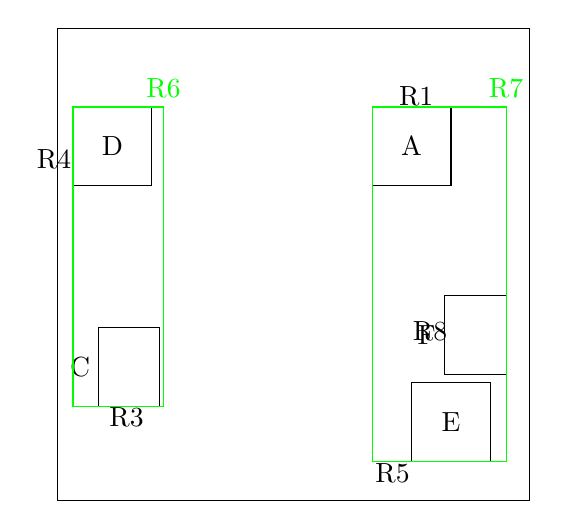
\begin{tikzpicture}
				% border
				\draw (0,0) rectangle (6,6);

				\nodeAA
				\nodeCC
				\nodeDD
				\nodeEE
				\nodeFF

				\RAA
				\RCC
				\RDD
				\REE
				\RFF

				% root node
				\draw[color=green] (0.2  , 1.2) rectangle (1.35, 5) node[anchor=south] {R6};
				\draw[color=green] (4.0, 0.5) rectangle (5.7, 5.0) node[anchor=south] {R7};
			\end{tikzpicture}
		\end{center}

		Einfügen von Eintrag G:
		\begin{center}
			\begin{tikzpicture}
				\draw (-1.5,0) rectangle (-0.5,1) node[name=R6,pos=.5] {R6};
				\draw (-0.5,0) rectangle (0.5,1) node[name=R7,pos=.5] {R7};
				\draw (0.5,0) rectangle (1.5,1) node[name=D1,pos=.5] {};
				\draw (1.5,0) rectangle (2.5,1) node[name=D2,pos=.5] {};

				\draw (-5,-2) rectangle (-4,-1) node[name=R1,pos=.5] {R3};
				\draw (-4,-2) rectangle (-3,-1) node[name=R3,pos=.5] {R4};
				\draw (-3,-2) rectangle (-2,-1) node[name=R5,pos=.5] {};
				\draw (-2,-2) rectangle (-1,-1) node[name=D3,pos=.5] {};

				\draw (1,-2) rectangle (2,-1) node[name=R2,pos=.5] {R1};
				\draw (2,-2) rectangle (3,-1) node[name=R4,pos=.5] {R5};
				\draw (3,-2) rectangle (4,-1) node[name=D4,pos=.5] {R8};
				\draw (4,-2) rectangle (5,-1) node[name=D5,pos=.5] {R9};

				\node[fit=(R1)(R3)(R5)(D3)](leftLeaf){};
				\node[fit=(R2)(R4)(D4)(D5)](rightLeaf){};

				\draw [thick, ->, >=stealth']
				([yshift=-2.5mm]R6.south) -- ([yshift=1mm]leftLeaf.north);
				\draw [thick, ->, >=stealth']
				([yshift=-2.5mm]R7.south) -- ([yshift=1mm]rightLeaf.north);
			\end{tikzpicture}
		\end{center}

		Die minimalen Rechtecke:
		\begin{center}
			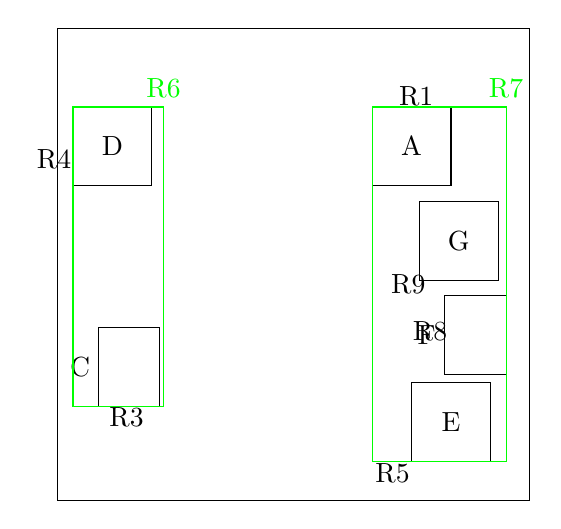
\begin{tikzpicture}
				% border
				\draw (0,0) rectangle (6,6);

				\nodeAA
				\nodeCC
				\nodeDD
				\nodeEE
				\nodeFF
				\nodeGG

				\RAA
				\RCC
				\RDD
				\REE
				\RFF
				\RGG

				% root node
				\draw[color=green] (0.2  , 1.2) rectangle (1.35, 5) node[anchor=south] {R6};
				\draw[color=green] (4.0, 0.5) rectangle (5.7, 5.0) node[anchor=south] {R7};
			\end{tikzpicture}
		\end{center}

		Einfügen von Eintrag H:
		\begin{center}
			\begin{tikzpicture}
				\draw (-1.5,0) rectangle (-0.5,1) node[name=R6,pos=.5] {R6};
				\draw (-0.5,0) rectangle (0.5,1) node[name=R7,pos=.5] {R7};
				\draw (0.5,0) rectangle (1.5,1) node[name=D1,pos=.5] {};
				\draw (1.5,0) rectangle (2.5,1) node[name=D2,pos=.5] {};

				\draw (-5,-2) rectangle (-4,-1) node[name=R1,pos=.5] {R3};
				\draw (-4,-2) rectangle (-3,-1) node[name=R3,pos=.5] {R4};
				\draw (-3,-2) rectangle (-2,-1) node[name=R5,pos=.5] {R10};
				\draw (-2,-2) rectangle (-1,-1) node[name=D3,pos=.5] {};

				\draw (1,-2) rectangle (2,-1) node[name=R2,pos=.5] {R1};
				\draw (2,-2) rectangle (3,-1) node[name=R4,pos=.5] {R5};
				\draw (3,-2) rectangle (4,-1) node[name=D4,pos=.5] {R8};
				\draw (4,-2) rectangle (5,-1) node[name=D5,pos=.5] {R9};

				\node[fit=(R1)(R3)(R5)(D3)](leftLeaf){};
				\node[fit=(R2)(R4)(D4)(D5)](rightLeaf){};

				\draw [thick, ->, >=stealth']
				([yshift=-2.5mm]R6.south) -- ([yshift=1mm]leftLeaf.north);
				\draw [thick, ->, >=stealth']
				([yshift=-2.5mm]R7.south) -- ([yshift=1mm]rightLeaf.north);
			\end{tikzpicture}
		\end{center}

		Die minimalen Rechtecke:
		\begin{center}
			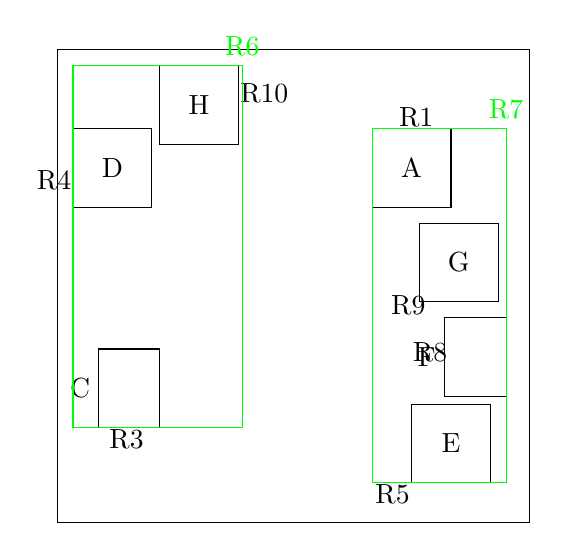
\begin{tikzpicture}
				% border
				\draw (0,0) rectangle (6,6);

				\nodeAA
				\nodeCC
				\nodeDD
				\nodeEE
				\nodeFF
				\nodeGG
				\nodeHH

				\RAA
				\RCC
				\RDD
				\REE
				\RFF
				\RGG
				\RHH

				% root node
				\draw[color=green] (0.2  , 1.2) rectangle (2.35, 5.8) node[anchor=south] {R6};
				\draw[color=green] (4.0, 0.5) rectangle (5.7, 5.0) node[anchor=south] {R7};
			\end{tikzpicture}
		\end{center}

		Einfügen von Eintrag I:
		\begin{center}
			\begin{tikzpicture}
				\draw (-1.5,0) rectangle (-0.5,1) node[name=R6,pos=.5] {R6};
				\draw (-0.5,0) rectangle (0.5,1) node[name=R7,pos=.5] {R7};
				\draw (0.5,0) rectangle (1.5,1) node[name=D1,pos=.5] {};
				\draw (1.5,0) rectangle (2.5,1) node[name=D2,pos=.5] {};

				\draw (-5,-2) rectangle (-4,-1) node[name=R1,pos=.5] {R3};
				\draw (-4,-2) rectangle (-3,-1) node[name=R3,pos=.5] {R4};
				\draw (-3,-2) rectangle (-2,-1) node[name=R5,pos=.5] {R10};
				\draw (-2,-2) rectangle (-1,-1) node[name=D3,pos=.5] {R11};

				\draw (1,-2) rectangle (2,-1) node[name=R2,pos=.5] {R1};
				\draw (2,-2) rectangle (3,-1) node[name=R4,pos=.5] {R5};
				\draw (3,-2) rectangle (4,-1) node[name=D4,pos=.5] {R8};
				\draw (4,-2) rectangle (5,-1) node[name=D5,pos=.5] {R9};

				\node[fit=(R1)(R3)(R5)(D3)](leftLeaf){};
				\node[fit=(R2)(R4)(D4)(D5)](rightLeaf){};

				\draw [thick, ->, >=stealth']
				([yshift=-2.5mm]R6.south) -- ([yshift=1mm]leftLeaf.north);
				\draw [thick, ->, >=stealth']
				([yshift=-2.5mm]R7.south) -- ([yshift=1mm]rightLeaf.north);
			\end{tikzpicture}
		\end{center}

		Die minimalen Rechtecke:
		\begin{center}
			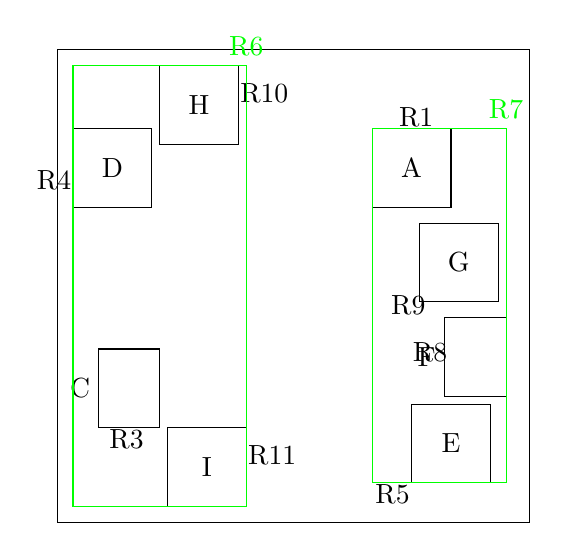
\begin{tikzpicture}
				% border
				\draw (0,0) rectangle (6,6);

				\nodeAA
				\nodeCC
				\nodeDD
				\nodeEE
				\nodeFF
				\nodeGG
				\nodeHH
				\nodeII

				\RAA
				\RCC
				\RDD
				\REE
				\RFF
				\RGG
				\RHH
				\RII

				% root node
				\draw[color=green] (0.2  , 0.2) rectangle (2.4, 5.8) node[anchor=south] {R6};
				\draw[color=green] (4.0, 0.5) rectangle (5.7, 5.0) node[anchor=south] {R7};

			\end{tikzpicture}
		\end{center}

		Einfügen von Eintrag J:
		\begin{center}
			\begin{tikzpicture}
				\draw (0,0) rectangle (1,1) node[name=R6,pos=.5] {R6};
				\draw (1,0) rectangle (2,1) node[name=R10,pos=.5] {R13};
				\draw (2,0) rectangle (3,1) node[name=R7,pos=.5] {R7};
				\draw (3,0) rectangle (4,1) node[name=D2,pos=.5] {};

				\draw (-5,-2) rectangle (-4,-1) node[name=R1,pos=.5] {R4};
				\draw (-4,-2) rectangle (-3,-1) node[name=R3,pos=.5] {R10};
				\draw (-3,-2) rectangle (-2,-1) node[name=R8,pos=.5] {R12};
				\draw (-2,-2) rectangle (-1,-1) node[name=D3,pos=.5] {};

				\draw (0,-2) rectangle (1,-1) node[name=R5,pos=.5] {R3};
				\draw (1,-2) rectangle (2,-1) node[name=R9,pos=.5] {R11};
				\draw (2,-2) rectangle (3,-1) node[name=D4,pos=.5] {};
				\draw (3,-2) rectangle (4,-1) node[name=D5,pos=.5] {};

				\draw (5,-2) rectangle (6,-1) node[name=D6,pos=.5] {R1};
				\draw (6,-2) rectangle (7,-1) node[name=D7,pos=.5] {R5};
				\draw (7,-2) rectangle (8,-1) node[name=D8,pos=.5] {R8};
				\draw (8,-2) rectangle (9,-1) node[name=D9,pos=.5] {R9};

				\node[fit=(R1)(R3)(R8)(D3)](leftLeaf){};
				\node[fit=(R5)(R9)(D4)(D5)](centerLeaf){};
				\node[fit=(D6)(D7)(D8)(D9)](rightLeaf){};

				\draw [thick, ->, >=stealth']
				([yshift=-2.5mm]R6.south) -- ([yshift=1mm]leftLeaf.north);
				\draw [thick, ->, >=stealth']
				([yshift=-2.5mm]R10.south) -- ([yshift=1mm]centerLeaf.north);
				\draw [thick, ->, >=stealth']
				([yshift=-2.5mm]R7.south) -- ([yshift=1mm]rightLeaf.north);
			\end{tikzpicture}
		\end{center}

		Die minimalen Rechtecke:
		\begin{center}
			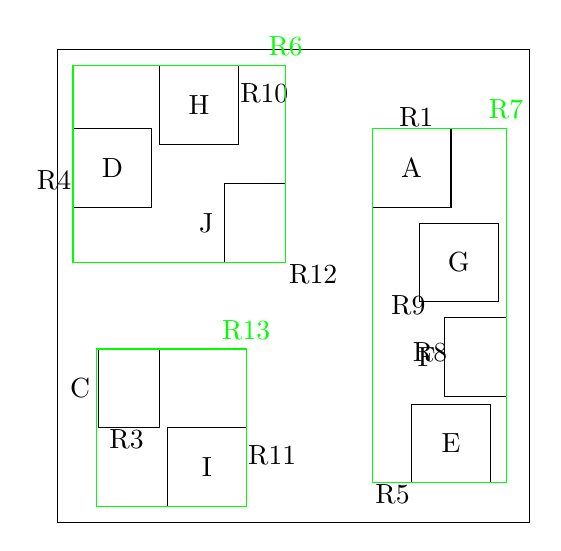
\begin{tikzpicture}
				% border
				\draw (0,0) rectangle (6,6);

				\nodeAA
				\nodeCC
				\nodeDD
				\nodeEE
				\nodeFF
				\nodeGG
				\nodeHH
				\nodeII
				\nodeJJ

				\RAA
				\RCC
				\RDD
				\REE
				\RFF
				\RGG
				\RHH
				\RII
				\RJJ

				% root node
				\draw[color=green] (0.2, 3.3) rectangle (2.9, 5.8) node[anchor=south] {R6};
				\draw[color=green] (4.0, 0.5) rectangle (5.7, 5.0) node[anchor=south] {R7};
				\draw[color=green] (0.5, 0.2) rectangle (2.4, 2.2) node[anchor=south] {R13};
			\end{tikzpicture}
		\end{center}
	\end{note}

	\item
	Löschen sie anschließend die Einträge D und I.

	\begin{note}
		Löschen von Eintrag D:
		\begin{center}
			\begin{tikzpicture}
				\draw (0,0) rectangle (1,1) node[name=R6,pos=.5] {R6};
				\draw (1,0) rectangle (2,1) node[name=R10,pos=.5] {R13};
				\draw (2,0) rectangle (3,1) node[name=R7,pos=.5] {R7};
				\draw (3,0) rectangle (4,1) node[name=D2,pos=.5] {};

				\draw (-5,-2) rectangle (-4,-1) node[name=R1,pos=.5] {R10};
				\draw (-4,-2) rectangle (-3,-1) node[name=R3,pos=.5] {R12};
				\draw (-3,-2) rectangle (-2,-1) node[name=R8,pos=.5] {};
				\draw (-2,-2) rectangle (-1,-1) node[name=D3,pos=.5] {};

				\draw (0,-2) rectangle (1,-1) node[name=R5,pos=.5] {R3};
				\draw (1,-2) rectangle (2,-1) node[name=R9,pos=.5] {R11};
				\draw (2,-2) rectangle (3,-1) node[name=D4,pos=.5] {};
				\draw (3,-2) rectangle (4,-1) node[name=D5,pos=.5] {};

				\draw (5,-2) rectangle (6,-1) node[name=D6,pos=.5] {R1};
				\draw (6,-2) rectangle (7,-1) node[name=D7,pos=.5] {R5};
				\draw (7,-2) rectangle (8,-1) node[name=D8,pos=.5] {R8};
				\draw (8,-2) rectangle (9,-1) node[name=D9,pos=.5] {R9};

				\node[fit=(R1)(R3)(R8)(D3)](leftLeaf){};
				\node[fit=(R5)(R9)(D4)(D5)](centerLeaf){};
				\node[fit=(D6)(D7)(D8)(D9)](rightLeaf){};

				\draw [thick, ->, >=stealth']
				([yshift=-2.5mm]R6.south) -- ([yshift=1mm]leftLeaf.north);
				\draw [thick, ->, >=stealth']
				([yshift=-2.5mm]R10.south) -- ([yshift=1mm]centerLeaf.north);
				\draw [thick, ->, >=stealth']
				([yshift=-2.5mm]R7.south) -- ([yshift=1mm]rightLeaf.north);
			\end{tikzpicture}
		\end{center}

		Die minimalen Rechtecke:
		\begin{center}
			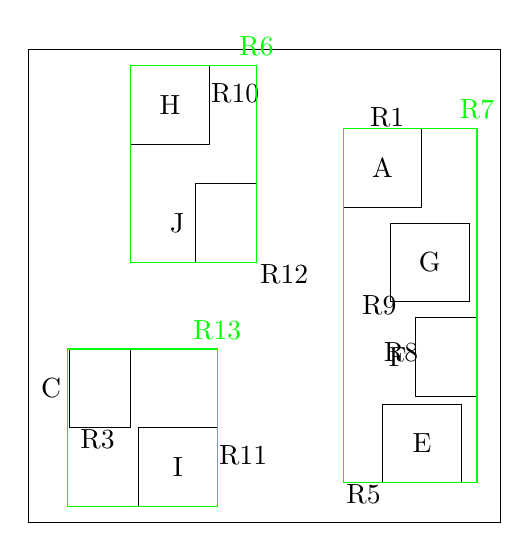
\begin{tikzpicture}
				% border
				\draw (0,0) rectangle (6,6);

				\nodeAA
				\nodeCC
				\nodeEE
				\nodeFF
				\nodeGG
				\nodeHH
				\nodeII
				\nodeJJ

				\RAA
				\RCC
				\REE
				\RFF
				\RGG
				\RHH
				\RII
				\RJJ

				% root node
				\draw[color=green] (1.3, 3.3) rectangle (2.9, 5.8) node[anchor=south] {R6};
				\draw[color=green] (4.0, 0.5) rectangle (5.7, 5.0) node[anchor=south] {R7};
				\draw[color=green] (0.5, 0.2) rectangle (2.4, 2.2) node[anchor=south] {R13};
			\end{tikzpicture}
		\end{center}

		Löschen von Eintrag I:
		\begin{center}
			\begin{tikzpicture}
				\draw (-1.5,0) rectangle (-0.5,1) node[name=R6,pos=.5] {R6};
				\draw (-0.5,0) rectangle (0.5,1) node[name=R7,pos=.5] {R7};
				\draw (0.5,0) rectangle (1.5,1) node[name=D1,pos=.5] {};
				\draw (1.5,0) rectangle (2.5,1) node[name=D2,pos=.5] {};

				\draw (-5,-2) rectangle (-4,-1) node[name=R1,pos=.5] {R3};
				\draw (-4,-2) rectangle (-3,-1) node[name=R3,pos=.5] {R10};
				\draw (-3,-2) rectangle (-2,-1) node[name=R5,pos=.5] {R12};
				\draw (-2,-2) rectangle (-1,-1) node[name=D3,pos=.5] {};

				\draw (1,-2) rectangle (2,-1) node[name=R2,pos=.5] {R1};
				\draw (2,-2) rectangle (3,-1) node[name=R4,pos=.5] {R5};
				\draw (3,-2) rectangle (4,-1) node[name=D4,pos=.5] {R8};
				\draw (4,-2) rectangle (5,-1) node[name=D5,pos=.5] {R9};

				\node[fit=(R1)(R3)(R5)(D3)](leftLeaf){};
				\node[fit=(R2)(R4)(D4)(D5)](rightLeaf){};

				\draw [thick, ->, >=stealth']
				([yshift=-2.5mm]R6.south) -- ([yshift=1mm]leftLeaf.north);
				\draw [thick, ->, >=stealth']
				([yshift=-2.5mm]R7.south) -- ([yshift=1mm]rightLeaf.north);
			\end{tikzpicture}
		\end{center}

		Die minimalen Rechtecke:
		\begin{center}
			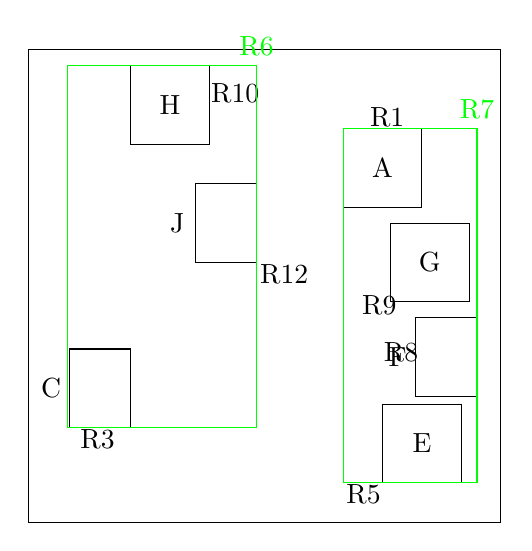
\begin{tikzpicture}
				% border
				\draw (0,0) rectangle (6,6);

				\nodeAA
				\nodeCC
				\nodeEE
				\nodeFF
				\nodeGG
				\nodeHH
				\nodeJJ

				\RAA
				\RCC
				\REE
				\RFF
				\RGG
				\RHH
				\RJJ

				% root node
				\draw[color=green] (0.5, 1.2) rectangle (2.9, 5.8) node[anchor=south] {R6};
				\draw[color=green] (4.0, 0.5) rectangle (5.7, 5.0) node[anchor=south] {R7};
			\end{tikzpicture}
		\end{center}
	\end{note}

\end{enumerate}
